
This chapter of the thesis will describe a MicroBooNE analysis done with the goal of constraining the intrinsic $\nu_e$ background for the previously described low energy excess search. As shown, this is the dominant background in the search, and a significant portion of the intrinsic $\nu_e$ background comes from kaon decay in the booster neutrino beam-line. The systematic uncertainty on the flux of $\nu_e$ from kaon decay is one of the largest uncertainties reducing the low energy excess significance. This chapter will describe how measuring the highest energy $\nu_\mu$ interactions in MicroBooNE can provide information about the kaon production in the beam-line, and constrain this important systematic. Exactly how these events are reconstructed and selected will be described, data to monte carlo comparisons will be shown, and the limitations of this analysis in its current form will be discussed.

%why we want to measure it, half of nues in search come from kaon decay, how to measure it is with high energy numus
%history: previous miniboone uncertainty on this was 40% or whatever, after gary's paper it's 14%,
%we want to explore doing the same measurement with microboone
%the general idea is to select high energy numus and compare data to MC to get a "normalization determination with improved uncertainty"
\section{BNB Kaon Production Introduction and Motivation}
As described in Chapter \ref{sec:beam}, the BNB is predominantly composed of $\nu_\mu$ (92.9\%) and $\overline{\nu}_\mu$ (6.5\%) with a small contamination of $\nu_e$ and $\overline{\nu}_e$ (0.6\% combined). The BNB flux by neutrino type at the MicroBooNE detector in neutrino-mode running is shown in Figure \ref{BNB_flux_uboone_fig}.

\begin{figure}[ht!]
\centering
	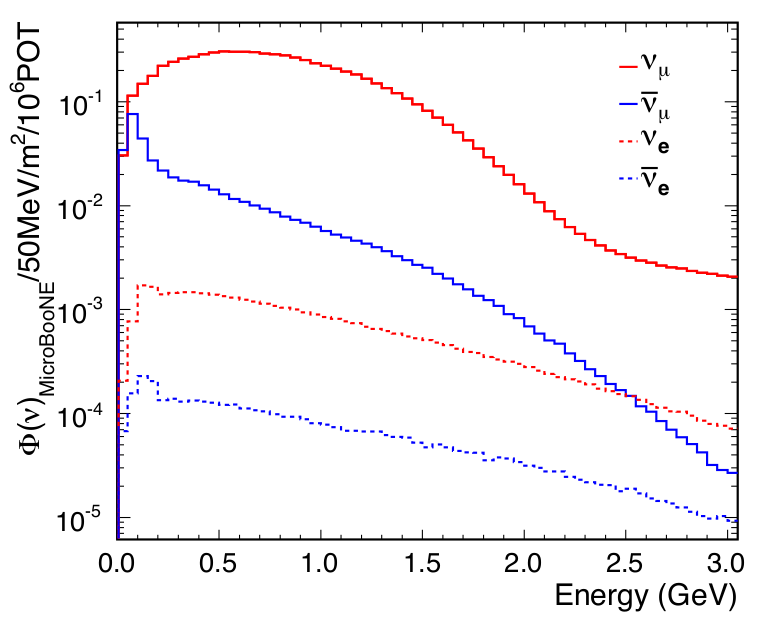
\includegraphics[width=0.9\textwidth]{Figures/BNB_flux_uboone.png} \\
\caption{\textit{The Booster Neutrino Beam (BNB) flux at MicroBooNE.}}\label{BNB_flux_uboone_fig}
\end{figure}

The decay modes producing beam $\nu_\mu$ and $\overline{\nu}_\mu$ are
\begin{itemize}
	\item $\pi^+\rightarrow\mu^++\nu_\mu$
	\item $K^+\rightarrow\mu^++\nu_\mu$
	\item $\pi^-\rightarrow\mu^-+\overline{\nu}_\mu$
\end{itemize}
and the decay modes producing beam $\nu_e$ and $\overline{\nu}_e$ are
\begin{itemize}
	\item $K^+ \rightarrow \pi^0 + e^+ + \nu_e$
	\item $\mu^+ \rightarrow e^+ + \overline{\nu}_\mu + \nu_e$
	\item $K^0_L \rightarrow \pi^- + e^+ + \nu_e$
	\item $K^0_L \rightarrow \pi^+ + e^- + \overline{\nu}_e$.
\end{itemize}

For the $\nu_\mu$ in the beam, the breakdown of $\nu_\mu$ production parentage as a function of neutrino energy is shown in Figure \ref{bnb_numu_breakdown_fig}. In the energy region $E_{\nu_\mu} < 2$ GeV, most $\nu_\mu$ come from $\pi^+$ decay, whereas at higher energies most $\nu_\mu$ come from $K^+$ decay. Therefore, the strategy to measure $K^+$ production in the beam is to select high energy $\nu_\mu$ interactions and compare simulation to data in terms of event rates in order to compute a normalization factor with an uncertainty.\\

\begin{figure}[ht!]
\centering
	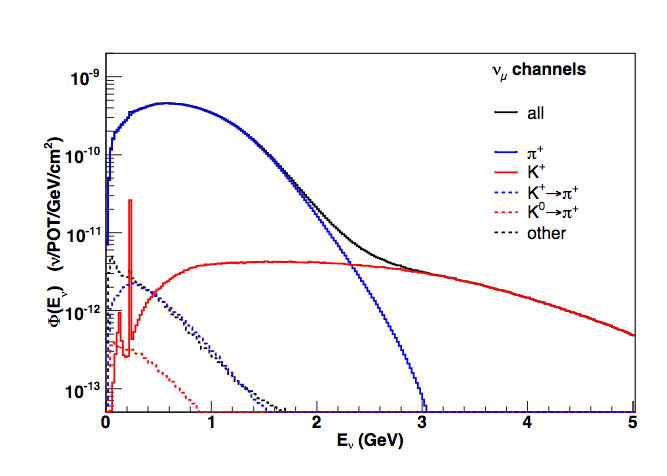
\includegraphics[width=0.9\textwidth]{Figures/bnb_numu_breakdown.png} \\
\caption{\textit{The beam $\nu_\mu$ parentage as a function of true neutrino energy.}}\label{bnb_numu_breakdown_fig}
\end{figure}

In the initial MiniBooNE publications, the systematic uncertainty on the intrinsic $\nu_e$ from $K^+$ decay in the beam was 40\%. This systematic came from several sources in the beam simulation process including proton delivery/optics, secondary particle productions, hadronic interactions in the target or horn, and horn magnetic field. The uncertainty in pion production was determined from spline fits to external HARP pion double differential cross section data using the Sanford-Wang (SW) parametrization \cite{SanfordWangGary7} \cite{HARPgary8}. There was no published external data for $K^+$ production at the BNB primary proton beam energy of 8 GeV, so the Feynman scaling hypothesis was used to extrapolate $K^+$ production measurements to this energy \cite{FEYNMANgary6}. Following a measurement by the SciBooNE collaboration \cite{gary_kaon_production_paper}, this uncertainty was reduced to 14\%. Even with this drastic reduction, $K^+$ production is still the largest source of uncertainty for BNB $\nu_e$ above neutrino energies of around 0.6 GeV, as shown in Figure \ref{UB_nue_fluxerror_fig}. The analysis described in the following sections aims to reproduce the SciBooNE measurement, but with the MicroBooNE detector. Reproducing this is important not only to further constrain this dominant systematic uncertainty for higher energy $\nu_e$ interactions, but also because MicroBooNE is has a different target material and different detector systematics. Additionally, the referenced analysis involved using the NUANCE neutrino interaction simulation library, whereas MicroBooNE uses a different package called GENIE.

\begin{figure}[ht!]
\centering
	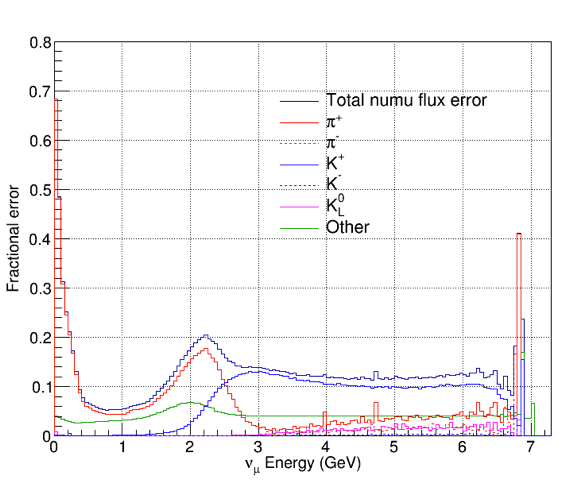
\includegraphics[width=0.9\textwidth]{Figures/UB_nue_fluxerror.png} \\
\caption{\textit{The fractional error for each neutrino species in the BNB at the MicroBooNE detector. Note the largest uncertainty at higher $\nu_\mu$ energies still comes from $K^+$ production, even including the SciBooNE measurement.}}\label{UB_nue_fluxerror_fig}
\end{figure}


\section{Event Selection}
The topologies of interest for this analysis are charge-current $\nu_\mu$ interactions in the MicroBooNE TPC. In such interactions, a $\nu_\mu$ interacts with a nucleon in an argon atom, exchanging a charged boson. Which particles exit the interaction depend on interaction channel and final state interactions, but in general these events have a muon in the final state. The relative probability of interaction type (quasi-elastic $QE$, resonant production $RES$, or deep inelastic scattering $DIS$) can be inferred from Figure \ref{bnb_xsec_breakdown_fig}. While most $\nu_\mu$ interactions in the dominant BNB energy region peaked at 0.7 GeV are quasi-elastic in nature, resonant production and deep inelastic scattering become more probable at higher neutrino energies.\\

\begin{figure}[ht!]
\centering
	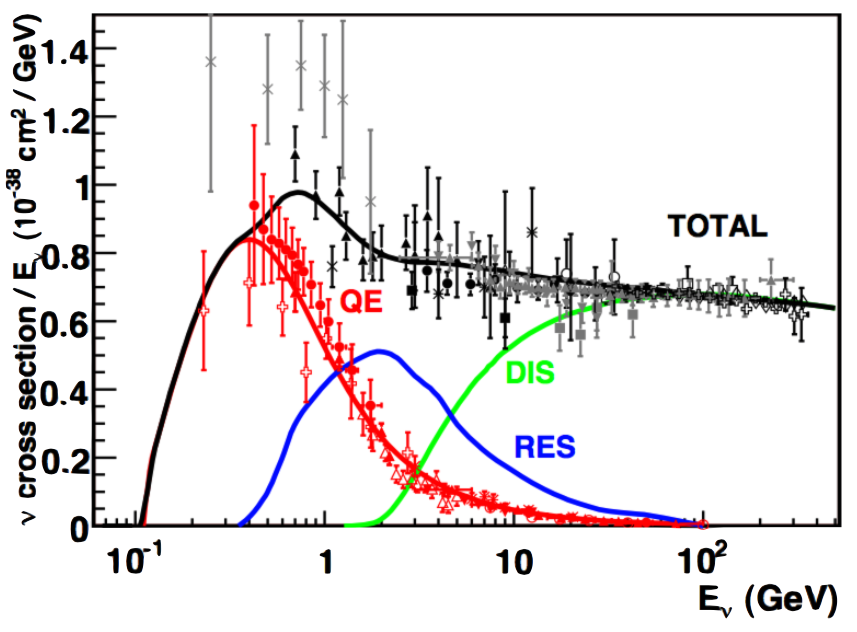
\includegraphics[width=0.9\textwidth]{Figures/numu_xsec_breakdown.png} \\
\caption{\textit{Muon neutrino charged-current cross section measurements and predictions as a function of neutrino energy.}}\label{bnb_xsec_breakdown_fig}
\end{figure}

The strategy is to select $\nu_\mu$ interaction events in MicroBooNE, reconstruct the neutrino energy, and then place a minimum energy cut to obtain a pure sample of $\nu_\mu$ events originating from kaon decay in the beam-line. The interaction reconstruction, selection criteria, and neutrino energy definition are described in the following subsections.

\subsection{Track Reconstruction}
This section provides a brief overview of how particles traversing the detector medium are physically observed and are reconstructed in software. For a thorough description of the MicroBooNE detector, see Section \ref{sec:detector}.\\

In a $\nu_\mu^{CC}$ (charge current) interaction, a muon exits the interaction vertex. This particle leaves a trail of ionization electrons that create a relatively straight-line pattern in three dimensions. This line of ionization electrons is referred to as a track. Other relevant particles traversing liquid argon that create tracks are protons and charged pions. These ionization electrons are drifted by an external electric field past three anode wire planes, situated at different angles, with 3 $mm$ spacing between each plane, and a 3 $mm$ pitch between each wire. Scintillation light from the particle is observed by photomultiplier tubes (PMTs) situated behind the anode wire planes. The signals observed on each wire plane provides a 2D image of the particle track, and combining information across multiple planes allows for complete 3D reconstruction, though there is ambiguity for the absolute location along the drift coordinate. Matching the timing of PMT signals with that of wire signals from a track clarifies this ambiguity, resulting in fully 3-dimensional reconstructed tracks.\\

The pattern recognition software used in this analysis to convert detector signals to reconstructed 3D tracks is called Pandora \cite{pandora_paper}. This package is responsible for taking reconstructed wire signals in a triggered MicroBooNE event, clustering them on each plane (with clusters representing individual particles in the event), and matching those clusters across planes to create 3D objects. In general, event reconstruction in a LArTPC is a difficult problem which the MicroBooNE collaboration has yet to fully solve. The Pandora package is a complex one which consists of a large number of nested algorithms designed to perform pattern recognition tasks, and these algorithms are not limited only to LArTPCs.\\

The output of the Pandora package that is relevant for this analysis are 3D reconstructed tracks created by Pandora's Projection Matching Algorithm (PMA), as well as 3D reconstructed interaction vertices which represent candidate neutrino interaction locations. Since $\nu_\mu^{CC}$ interactions always have a muon track exiting an interaction vertex, this is the fundamental criteria to select a sample of these events. More detailed criteria are needed to mitigate backgrounds, and the selection cuts are described in more detail in the following section.

\subsection{Selection Criteria}\label{kaon_event_selection_section}
The following selection criteria are placed on the reconstructed objects to select $\nu_\mu$ charged-current interactions in which a candidate muon track exits the interaction vertex:

\begin{enumerate}
\item The event must have at least one bright (50 photoelectron equivalent) optical flash, reconstructed from PMT timing signals, in coincidence with the expected BNB-neutrino arrival time. %1
\item The $z$ coordinate of the optical flash, as determined by the pulse height and timing of signals in the 32 PMTs, must be within 70 cm of any point on the $z$ projection of the candidate muon track. %2 
\item Two or more reconstructed tracks must originate from the same reconstructed vertex within the fiducial volume. %3
\item For events with exactly two tracks originating from the vertex, additional calorimetric criteria are applied to mitigate backgrounds from cosmic muons that arrive in time with the passage of the beam, then stop and decay to an electron that is reconstructed as a track. %4   
\item The length of the longest track associated with the interaction must be at least 15 centimeters in length.
\item For events with exactly two tracks originating from the same reconstructed vertex must not have exactly opposite directions (to within 5 degrees).
\end{enumerate}

Selection criteria (1) and (2) are necessary to mitigate backgrounds originating from cosmic rays arriving in coincidence with the expected beam-neutrino arrival time and triggering a readout. \\

Selection criteria (3) is necessary to mitigate cosmic backgrounds. Cosmics entering from outside of the TPC will often lead to reconstructed neutrino vertices very close to the TPC boundaries. The boundaries of the fiducial volume used in this analysis are set back from the six faces of the active volume by distances of between 20 and 37 cm, depending on the face. This volume was also chosen to reduce the impact of electric-field non-uniformities near the edges of the TPC \cite{SCE_publicnote}, which are relevant when reconstructing a track energy (described in the next section). The fiducial volume corresponds to a mass of 55 tons.\\

Selection criteria (3) is also necessary to address mis-identifications stemming from track reconstruction failures. There exists a sizable background in which a cosmic traverses the entire detector, but only a portion of its track gets reconstructed, mimicking the one-track topology. These one-track events are removed at the cost of $\nu_\mu^{CCQE}$ interactions in which only a muon exits the interaction vertex. Given that this analysis geared towards the highest energy $\nu_\mu$ interactions which are often in the RES or DIS channel (multi-track), this cut isn't very detrimental to the desired high neutrino energy signal.\\

Selection criteria (4) is necessary to remove the specific topology where a cosmic ray muon stops in the detector (with an increased ionization rate as it approaches its endpoint, known as a Bragg peak) and subsequently decays into an electron. This topology has two tracks exiting a ``kink'', which mimics a $\nu_\mu^{CC}$ topology. This cut leverages the presence of the Bragg peak to correctly identify the directions of the two tracks and therefore remove this event from the analysis.\\

Selection criteria (5) and (6) are additional cuts to mitigate specific track reconstruction failure modes that are present when reconstructing cosmic rays. In these failure modes, a long straight track can be broken up and reconstructed as two or more straight tracks, with a reconstructed vertex as the breaking point.\\

The above selection criteria serve only to select a sample of $\nu_\mu^{CC}$ events, which come from both pion and kaon decay. The efficiency to select events these is defined as
\begin{equation}
\epsilon_{\nu_\mu^{CC}} = \frac{\text{\# selected events}}{\text{\# true $\nu_\mu^{CC}$ events in the fiducial volume}}
\end{equation}
and the purity is defined as
\begin{equation}
\pi_{\nu_\mu^{CC}} = \frac{\text{\# true $\nu_\mu^{CC}$ correctly identified events in selected sample}}{\text{\# selected events}}.
\end{equation}
With the described selection criteria, the efficiency $\epsilon_{\nu_\mu^{CC}}$ is 27\%. This efficiency is rather low because of the requirement of two reconstructed tracks exiting the interaction combined with a low track reconstruction efficiency, especially for short tracks near the vertex. The purity is 82\%, and the primary contaminating backgrounds are those from cosmics. The backgrounds to this analysis are discussed in more detail in the following section.

\subsection{Backgrounds}
There are three main backgrounds to this $\nu_\mu^{CC}$ from $K^+$ decay search: $\nu_\mu^{CC}$ from $\pi$ decay interactions, neutral current interactions, and cosmic-induced backgrounds. The $\nu_\mu^{CC}$ from $\pi$ decay interactions are the most dominant background and will be removed with a cut on neutrino energy, which is described in the following section.\\

The neutral current backgrounds occur when a beam neutrino of any flavor interacts in such a way as to mimic a $\nu_\mu^{CC}$ interaction. For example, a neutrino can interact with a nucleus and liberate a proton and a charged pion. In this case, the charged pion may be mis-identified as a muon.\\ %Additionally, a neutrino may interact and create a neutral pion which subsequently decays into two photon showers. It is possible those showers accidentally get reconstructed as tracks, mimicking a $\nu_\mu^{CC}$ interaction.\\

The cosmic-induced backgrounds are mitigated largely by the previously described event selection cuts. Their topologies are usually caused either by track reconstruction failures, or by stopping muons which decay into electrons. In the latter example, the track direction of the muon must be incorrect, and the decay electron must be reconstructed as a separate track. Though many calorimetric and track-length based selection criteria are used to reduce this background, it still persists because the rate of stopping cosmics in triggered readouts far outweighs that of $\nu_\mu^{CC}$ interactions.\\

With the events selected, the next step is to reconstruct the neutrino energy. This is necessary because the neutrino energy is the variable through which the $\nu_\mu$ from $K^+$ decay sample of interest is isolated.

\section{Neutrino Energy Reconstruction}\label{kaon_nu_energy_section}

Event selection (Section \ref{kaon_event_selection_section}) provides a sample of candidate $\nu_\mu^{CC}$ interactions consisting of a number ($>2$) of reconstructed tracks exiting a common neutrino interaction vertex. Each track must first be associated with a particle identity (referred to as PID) in order to compute the energy of that track. Note that in $\nu_\mu^{CC}\pi^0$ interactions there will also be two showers exiting the vertex from the neutral pion decay. However, these showers (and therefore their associated energy) are ignored. The reason for this is that at the time of this analysis, the shower reconstruction performance in MicroBooNE software isn't at an adequate level to include them. Excluding them will ultimately worsen the energy reconstruction performance, but the performance is still sufficient to select a pure sample of $\nu_\mu^{CC}$ interactions from $K^+$ decay, as will be shown later.\\

The longest track in this set is assumed to be the muon, which is reasonable because on average the majority of the neutrino energy in a $\nu_\mu^{CC}$ interaction is transferred to the outgoing muon, as shown in Figure \ref{numuCC_energyfraction_tomuon_fig}. Also, muons are in general closer to minimally ionizing than to other final state particles like protons and therefore produce the longest tracks.\\

\begin{figure}[ht!]
\centering
	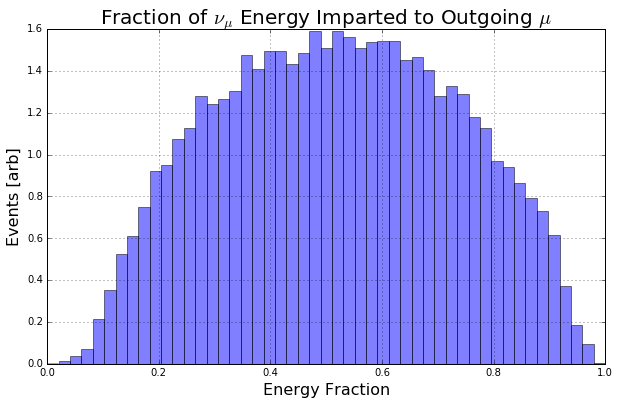
\includegraphics[width=0.9\textwidth]{Figures/numuCC_energyfraction_tomuon.png} \\
\caption{\textit{The fraction of $\nu_\mu$ energy imparted to the outgoing lepton ($\mu$) in $\nu_\mu^{CC}$ interactions.}}\label{numuCC_energyfraction_tomuon_fig}
\end{figure}

The remaining tracks exiting the interaction are classified as either charged pions, or protons. This is reasonable because only one muon can exit a $\nu_\mu^{CC}$ interaction vertex (barring negligibly rare topologies in which a charged pion is created and decays within the nucleus, resulting in two muons in the final state). Protons are much more highly ionizing than charged pions, and therefore the measured dE/dx of the tracks are used in classification; shorter, highly ionizing tracks are tagged as protons, and longer, lower ionizing tracks are tagged as charged pions.\\

The reconstructed neutrino energy is defined as the sum of the energies of all tracks exiting the interaction vertex. For muon and pion tracks, their total energies are added (including mass), while for proton tracks only the kinetic energy is added. This is because while the muons and pions are created with energy directly from the neutrino, the protons are pre-existing and are liberated from the nucleus. This simplistic energy definition neglects binding energy in the nucleus, but that effect is small.\\

The method used to reconstruct the energy of the muon track depends on whether that track is fully contained in the fiducial volume. In general, reconstructing the energies of fully contained particle tracks in a LArTPC is straightforward, either with a range-based approach, or a calorimetric approach (since calorimetric information can be gleaned from the size of sense-wire signals). In this analysis, range-based energy is used for fully contained muons. The stopping power of muons in liquid argon is well described by the continuous slowing-down approximation (CSDA) by the particle data group, and agrees with data at the sub-percent level \cite{MIPenergysource} \cite{PDG_spline_table}. By using a linear interpolation between points in the stopping power table of ref. \cite{PDG_spline_table}, the length of a track can be used to reconstruct the muon's total energy with resolution better than 4\% and negligible bias.\\

For muon tracks that exit the fiducial volume (which is ultimately the case for all selected $\nu_\mu^{CC}$ from $K^+$ decay), a different method is required to compute the track energy. This method leverages a phenomenon called multiple Coulomb scattering (MCS), and the development and characterization of this method is the subject of a pending publication by the author of this thesis in the Journal of Instrumentation. This publication comprises the following chapter of this thesis. To summarize, the MCS energy resolution for well reconstructed exiting muon tracks with at least one meter of their length contained in the fiducial volume is on the order of 15\% for muons with momenta below 2.5 GeV/c, and on the order of 30\% for muons with momenta between 2.5 and 4.0 GeV/c. A downside to the MCS method is that it requires at least a meter of track to be contained. For muons that exit with less than a meter contained, the range-based energy is necessarily used, which is often a significant underestimation of the true energy. Note that space charge effects most predominantly located near the edges of the TPC are not included in this simulation. These electric-field non-uniformities have the effect of bending a track, which will cause the MCS technique to underestimate the track's energy. To account for this difference between data and Monte-Carlo, all reconstructed tracks in this analysis are truncated to be contained within the fiducial volume, which was chosen because the effect of electric field non-uniformities are small in this region. This effectively converts the fiducial volume to an active volume, in which space charge effects are negligible.\\

Charged pion tracks are treated in much the same way as muon tracks. When they are contained, range-based energy is used, and when they exit, MCS energy is used (despite the fact that MCS energy is tuned for muons, the same method works sufficiently well for the purposes of this analysis on pions). Proton tracks are in general much shorter and therefore their probability of exiting the fiducial volume is small. For these tracks, a range-based energy is used based on the stopping power of protons in liquid argon published by the same aforementioned references.\\

Given the described event selection criteria, particle identification techniques, and track energy methods, a distribution of the reconstructed neutrino energy versus true neutrino energy for a sample of correctly identified $\nu_\mu^{CC}$ interactions in MicroBooNE simulation is shown in Figure \ref{kaon_recoenergy_2d_fig}. It can be seen that the reconstructed energy tends to be an underestimation of the true energy. This is caused by the failure to include shower-based energy from the interaction (as mentioned previously), as well as needing to use range-based energy for tracks which have less than one meter contained in the TPC. Additionally the relatively crude particle identification techniques could have an impact as well. While this reconstructed neutrino energy could certainly be improved upon, its performance is sufficient for this analysis. As you can see from the figure, placing a cut on reconstructed neutrino energy at around 2.5 GeV will provide a relatively pure sample of events in which the true neutrino energy is also above 2.5 GeV. Since this analysis is a normalization measurement (a counting experiment), the shortcomings of this neutrino energy definition are acceptable.

\begin{figure}[ht!]
\centering
	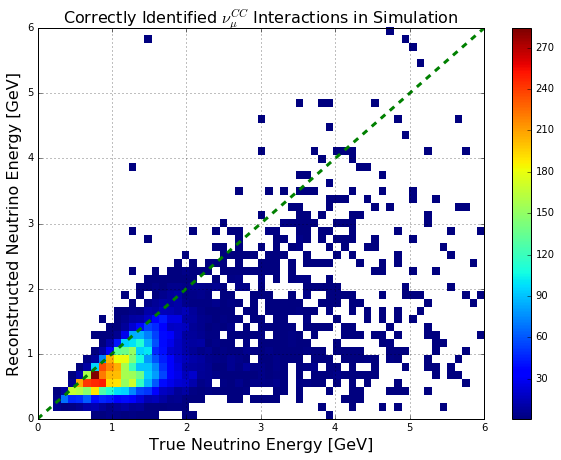
\includegraphics[width=0.9\textwidth]{Figures/kaon_recoenergy_2d.png} \\
\caption{\textit{Reconstructed neutrino energy versus true neutrino energy for a sample of correctly identified BNB $\nu_\mu^{CC}$ interactions in the MicroBooNE TPC.}}\label{kaon_recoenergy_2d_fig}
\end{figure}

\section{Results in Simulation}
The simulation used for this analysis are BNB simulated neutrino interactions within the entire MicroBooNE TPC. The BNB flux is described in Chapter \ref{sec:beam} of this thesis. The neutrino interaction event generator used is GENIE \cite{GENIEsource}. These interactions also include simulated cosmic rays by the CORSIKA package \cite{CORSIKAsource}. This ``BNB + Cosmic'' simulation provides the measurement sample as well as all relevant backgrounds. If a reconstructed neutrino vertex is within 3 cm of a true $\nu_\mu^{CC}$ interaction vertex, that event will be classified as either $\nu_\mu$ from pion decay (background) or $\nu_\mu$ from kaon decay (signal), depending on the true neutrino parent. If the reconstructed neutrino vertex is within 3 cm of a true $\nu_x^{NC}$ interaction vertex, that event is classified as a neutral current background. Lastly, if the reconstructed neutrino vertex is not near any true neutrino interaction point, the interaction is tagged as cosmic.\\

2.2 $\times 10^{20}$ protons-on-target are simulated in this analysis, and the final histograms are scaled to 0.5 $\times 10^{20}$. This scaling is done because when a comparison to data is made (in the next section), only 0.5 $\times 10^{20}$ protons-on-target worth of data are available for this analysis due to blinding schemes within the MicroBooNE collaboration. Note that the nominal amount of protons-on-target scheduled to be delivered to MicroBooNE over a three-year running period is much more than this, 6.6$\times 10^{20}$; unblinding the full data set in the future will improve the strength of this analysis' result by decreasing the statistical uncertainty. \\

The distribution of simulated signal and backgrounds as a function of reconstructed neutrino energy between 0 and 2.5 GeV (which is referred to as the sideband region for this analysis) in Figure \ref{kaon_stack_sideband_nodata}. In this stacked histogram figure, the green histogram is the signal of interest, $\nu_\mu^{CC}$ interactions from kaon decay. In this sideband region the $\nu_\mu^{CC}$ from pion decay (blue) is the dominant background, while cosmic-induced backgrounds (red) are mostly relevant at reconstructed neutrino energies below 1 GeV. Neutral current backgrounds (yellow) are sub-dominant.\\

\begin{figure}[ht!]
\centering
	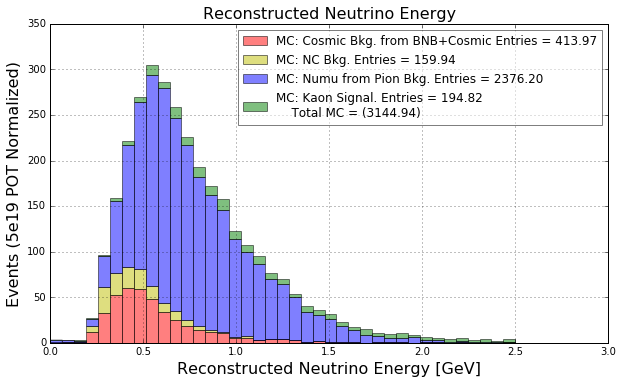
\includegraphics[width=0.9\textwidth]{Figures/kaon_simonly_sideband.png} \\
\caption{\textit{Distribution of signal (green) and backgrounds normalized for 0.5 $\times 10^{20}$ protons-on-target worth of data, for reconstructed neutrino energy below 2.5 GeV. This comprises the sideband region.}}\label{kaon_stack_sideband_nodata}
\end{figure}

In order to select a relatively pure sample of $\nu_\mu^{CC}$ from $K^+$ decay interactions, a cut on reconstructed neutrino energy is placed at 2.5 GeV. The resulting sample has a kaon signal purity of 81\%, and is shown in Figure \ref{kaon_stack_signal_nodata}. In this region, the backgrounds from neutral current interactions and from $\nu_\mu^{CC}$ from $\pi$ decay are drastically suppressed. Still remaining is a cosmic-induced background which comprises 15\% of the sample. The correlation between energy and angle of the kaons which decay to produce $\nu_\mu^{CC}$ interactions in the fiducial volume is shown in Figure \ref{all_kaon_energy_angle_2d}, and the subset of those which are reconstructed and selected in this analysis (passing the 2.5 GeV cut on neutrino energy) are shown in Figure \ref{selected_kaon_energy_angle_2d}. The projection of these distributions onto the angle axis are shown in Figure \ref{kaon_angle_selection}, and onto the energy axis in Figure \ref{kaon_energy_selection}. The mean energy and angle information for kaons which produce $\nu_\mu$ (all, and selected) and for those which produce $\nu_e$ (relevant for the electron-like low energy excess analysis) are summarized in Table \ref{kaon_energy_angle_table}. The kaons selected in the signal region tend to be skewed towards being more forward-going (smaller angle) and having higher energy, though the production phase-space is still reasonably covered by the selection (as seen by comparing Figures \ref{all_kaon_energy_angle_2d} and \ref{selected_kaon_energy_angle_2d}).
% XXX here i discuss that we use genie whereas sciboone used NUANCE which is an important difference. also mention that the simulated samples are BNB+cosmic overlayed with corsika, each event has neutrino interaction in it and associated POT. describe how in real data only like 1/6 triggers have a neutrino, and describe how we handle the relative normalization of that (beam on minus beam off).

%

\begin{figure}[ht!]
\centering
	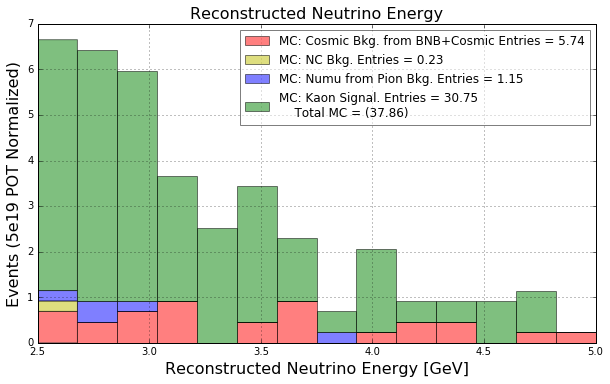
\includegraphics[width=0.9\textwidth]{Figures/kaon_simonly_signal.png} \\
\caption{\textit{Distribution of signal (green) and backgrounds normalized for 0.5 $\times 10^{20}$ protons-on-target worth of data, for reconstructed neutrino energy between 2.5 GeV and 5 GeV. This comprises the signal region, which has an 81\% purity of $\nu_\mu^{CC}$ interactions from $K^+$ decay in the beam.}}\label{kaon_stack_signal_nodata}
\end{figure}


\begin{figure}[ht!]
\centering
	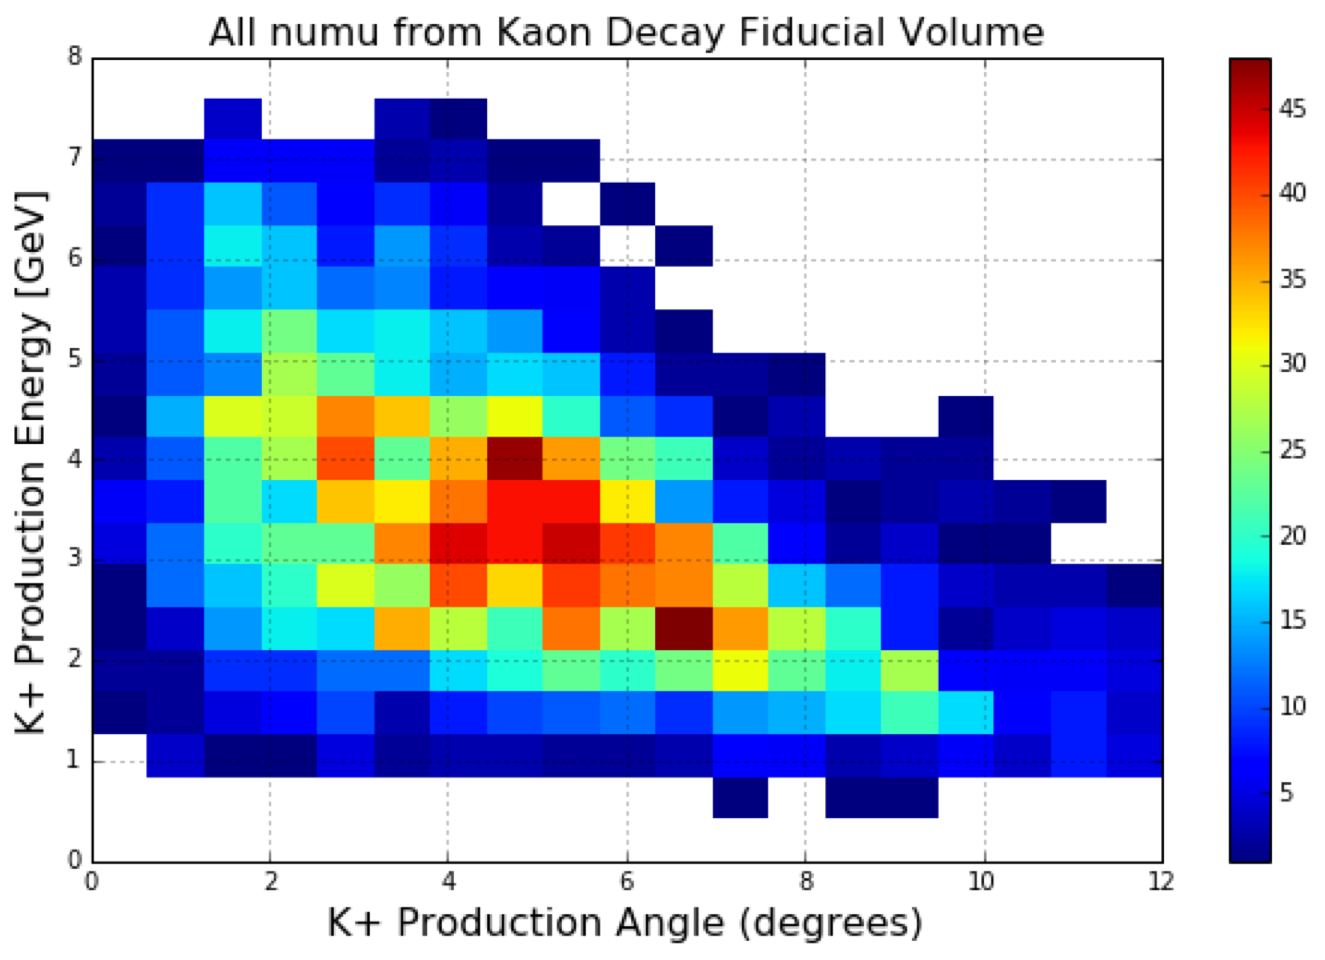
\includegraphics[width=0.9\textwidth]{Figures/all_kaon_energy_angle_2d.png} \\
\caption{\textit{A two-dimensional plot of energy versus angle for all kaons in the beam producing $\nu_\mu^{CC}$ interactions in the detector.}}\label{all_kaon_energy_angle_2d}
\end{figure}


\begin{figure}[ht!]
\centering
	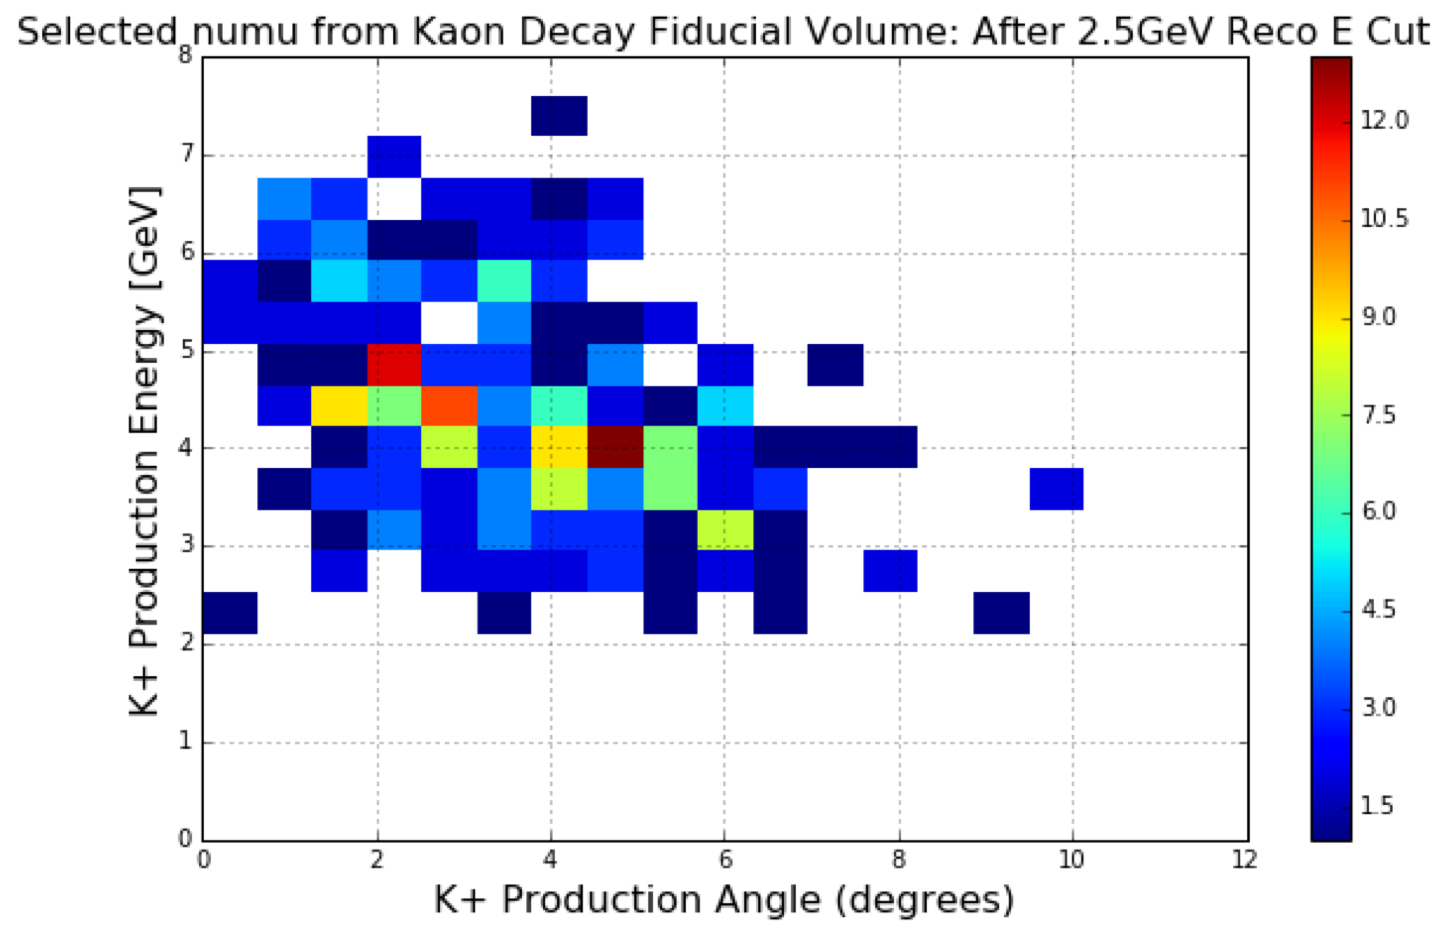
\includegraphics[width=0.9\textwidth]{Figures/selected_kaon_energy_angle_2d.png} \\
\caption{\textit{A two-dimensional plot of energy versus angle for the subset of kaons in Figure \ref{all_kaon_energy_angle_2d} which are reconstructed and selected for this analysis (having reconstructed neutrino energy above 2.5 GeV).}}\label{selected_kaon_energy_angle_2d}
\end{figure}


\begin{figure}[ht!]
\centering
	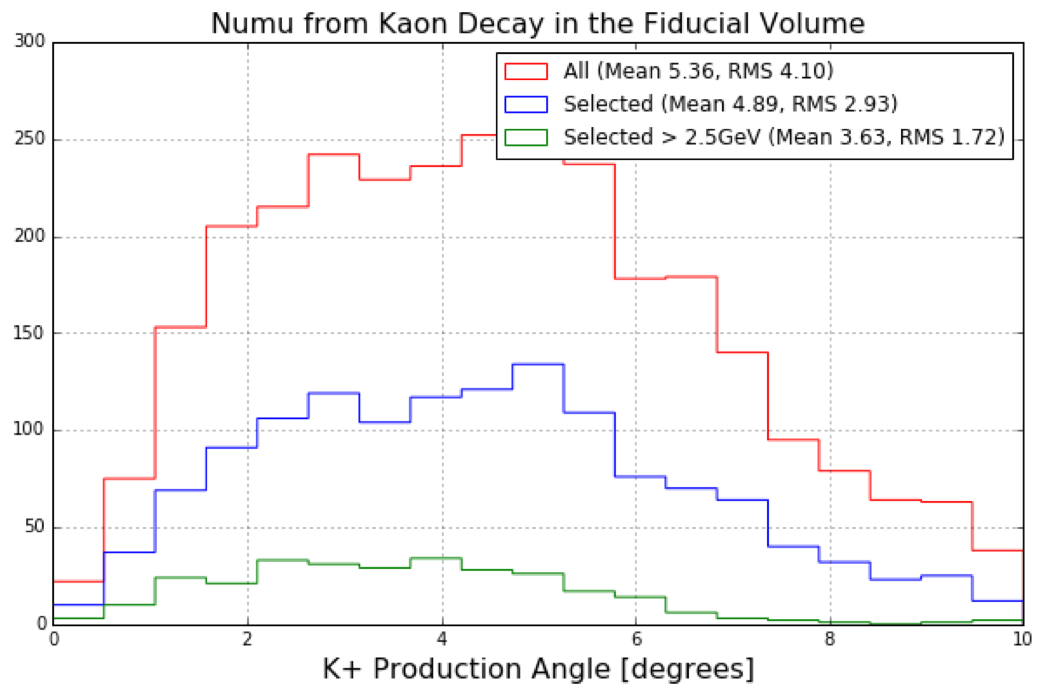
\includegraphics[width=0.9\textwidth]{Figures/kaon_angle_selection.png} \\
\caption{\textit{The kaon production angle distribution for all kaons in the beam producing $\nu_\mu^{CC}$ interactions in the detector (red), the subset of those which are reconstructed and selected in both the sideband and signal region (blue) and the subset of those in the Kaon enriched signal sample, with reconstructed neutrino energy above 2.5 GeV (green).}}\label{kaon_angle_selection}
\end{figure}


\begin{figure}[ht!]
\centering
	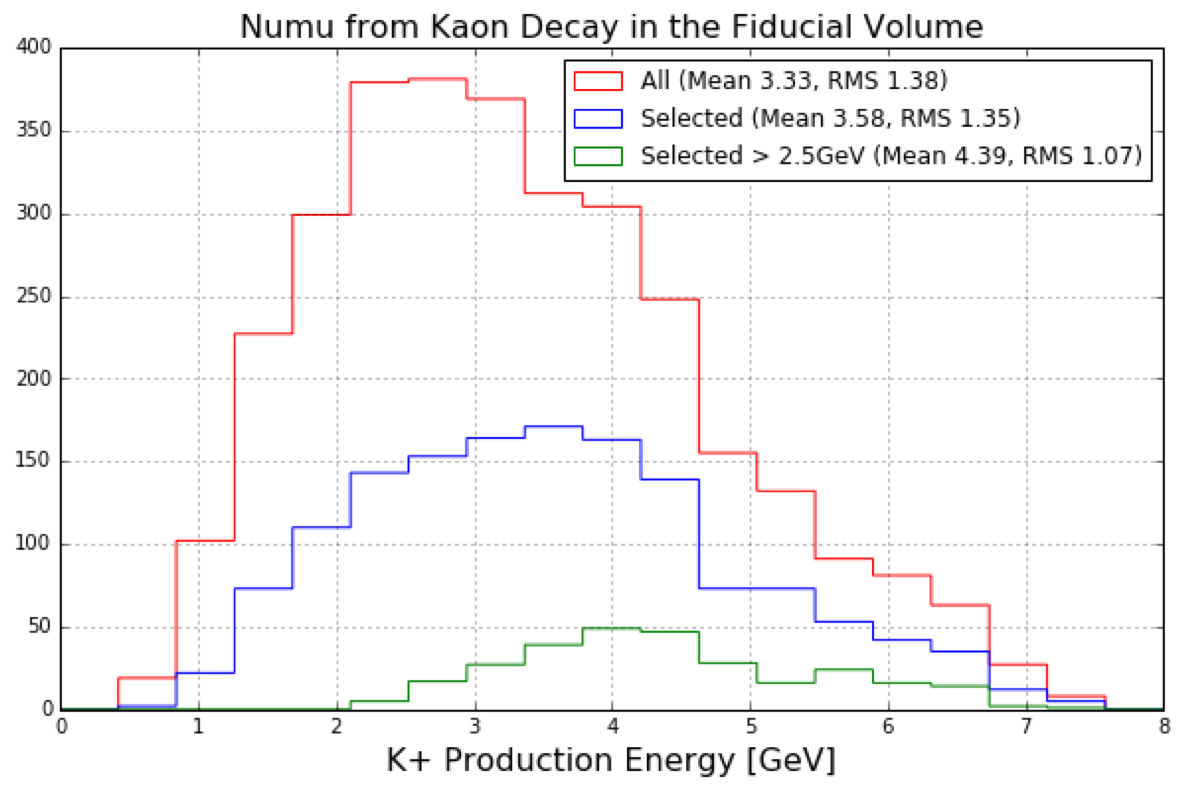
\includegraphics[width=0.9\textwidth]{Figures/kaon_energy_selection.png} \\
\caption{\textit{The kaon production energy distribution for all kaons in the beam producing $\nu_\mu^{CC}$ interactions in the detector (red), the subset of those which are reconstructed and selected in both the sideband and signal region (blue) and the subset of those in the Kaon enriched signal sample, with reconstructed neutrino energy above 2.5 GeV (green).}}\label{kaon_energy_selection}
\end{figure}


\begin{table}
\begin{tabular}{ |p{0.5cm}|p{2.5cm}|p{4cm}|p{3cm}|p{3.5cm}|  }
 \hline
 \multicolumn{5}{|c|}{Kaon Production Summary} \\
 \hline
   & All $\overline{K_\theta}$ [deg] & Selected $\overline{K_\theta}$ [deg] & All $\overline{K_E}$ [GeV] & Selected $\overline{K_E}$ [GeV]\\
 \hline \hline
 $\nu_\mu$ & 5.36 [4.10] & 3.63 [1.72] & 3.33 [1.38] & 4.39 [1.07] \\\hline
 $\nu_e$ & 5.10 [3.68] & N/A & 3.32 [1.28] & N/A \\\hline
 \hline
\end{tabular}
\caption{\textit{A summary of the mean kaon production angle ($\overline{K_\theta}$) and energy ($\overline{K_E}$) in the BNB for $\nu_\mu$ interactions (all interactions interacting within the TPC, and the subset of those which are selected in the analysis), and for $\nu_e$ interactions (providing backgrounds to the electron-like low energy excess search). Reported in brackets is the RMS of each distribution.}}\label{kaon_energy_angle_table}
\end{table}


















\section{Sideband Data and Simulation Comparisons}
As shown in the previous section, the event reconstruction and selection is able to provide a relatively pure signal sample of $\nu_\mu^{CC}$ from kaon decay interactions in the detector by choosing those with reconstructed neutrino energy above 2.5 GeV. While the sideband region (with reconstructed neutrino energy below 2.5 GeV) is composed primarily of backgrounds from $\nu_\mu^{CC}$ from $\pi$ decay interactions, it is used for lower-level comparisons between data and simulation to increase confidence in results from the signal region. This section will show several such comparison plots.\\

In order to compare data to simulation, there is a subtlety involving the cosmic background which needs to be accounted for. In the simulation, each triggered readout event has a neutrino interacting somewhere within the TPC, along with several simulated cosmic rays. However, in real data, the majority of triggers are induced by cosmic interactions arriving during the expected neutrino arrival timing window ($1.6\mu s$), and do not contain a neutrino interaction at all. To account for this, a sample of data is taken when the neutrino beam is turned off, in order to get an estimate of the cosmic background. This ``off-beam'' data is then subtracted from the ``on-beam'' data in the analysis, and the difference is what is directly comparable to simulation. The normalization factor between ``off-beam'' and ``on-beam'' data is computed based on the number of measured bright reconstructed optical flashes within the expected neutrino arrival window both during ``off-beam'' (cosmic-only) runs and ``on-beam'' runs. This factor is computed to be 0.844, which means that 84\% of triggered BNB readouts relevant to this analysis in MicroBooNE data are cosmic-induced. Note that while subtracting ``off-beam'' data from ``on-beam'' data accounts for the cosmic backgrounds not taken included in simulation, there still exists a cosmic background originating from readouts which are truly triggered by a neutrino interaction, but a cosmic arriving during the milliseconds-long readout window is mistakenly identified as the neutrino interaction. This is the background shown in red in the previously shown stacked histograms. In the forthcoming data-MC comparison plots, the ``off-beam'' data points are shown in cyan for reference only; they are already subtracted from the ``on-beam'' data when they are drawn in purple.\\

The first low level data to simulation comparison done in the sideband region is shown in Figure \ref{kaon_sideband_comp_tracklength}. This plot shows the simulated background and signals as a stacked histogram with the same color-coding as shown previously (Figure \ref{kaon_stack_sideband_nodata}). Shown in cyan is this distribution for events selected from ``off-beam'' data, which are purely cosmic mis-identifications. These points are shown only for reference. The purple data points represent ``on-beam'' minus ``off-beam'' distributions and therefore already have the cyan points subtracted out. Statistical error bars are drawn on the purple data points, taking into account statistics from both the ``on-beam'' and ``off-beam'' samples. We see a normalization difference between data and simulation of about 8\%, with data having fewer events than expected in simulation. This normalization difference in the sideband serves as a calibration factor to be applied to the signal region. Below the main figure is a bin-by-bin ratio plot of data divided by simulation. The agreement is reasonable for this variable, with the ratio generally agreeing with unity to within (statistical) uncertainty.\\


\begin{figure}[ht!]
\centering
	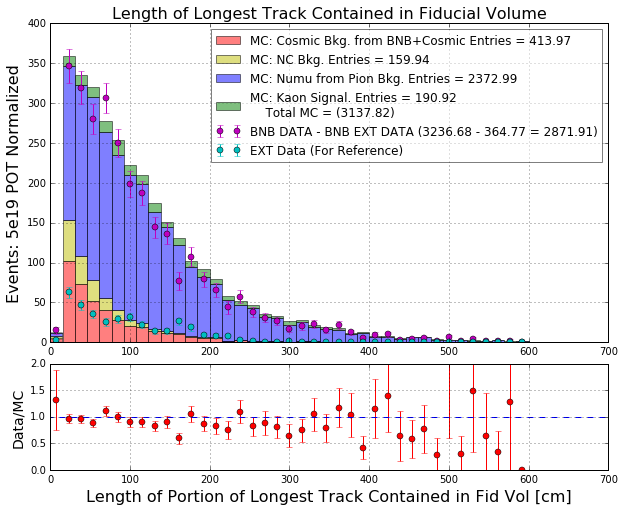
\includegraphics[width=0.9\textwidth]{Figures/kaon_sideband_comp_tracklength.png} \\
\caption{\textit{The distribution of length of the longest track associated with the interaction contained within the fiducial volume for simulated backgrounds and signal (solid histograms) overlaid with data measurements (``on-beam'' minus ``off-beam'' drawn in purple) for the sideband region in which reconstructed neutrino energy is less than 2.5 GeV. Statistical error bars are drawn on the data points, taking into account statistics from both the ``on-beam'' and ``off-beam'' samples.}}\label{kaon_sideband_comp_tracklength}
\end{figure}

The next low-level data to simulation comparison in the sideband region is shown in Figure \ref{kaon_sideband_comp_multiplicity}. This is the track multiplicity (the number of reconstructed tracks associated with the interaction). The same normalization offset of 8\% persists (since these are the same events as in Figure \ref{kaon_sideband_comp_tracklength}). While data and simulation agree for three-track events, they begin to disagree for other multiplicities. The reason for this could be imperfect modeling of nuclear interactions (including final-state intra-nuclear interactions) within the neutrino interaction simulation package.\\

\begin{figure}[ht!]
\centering
	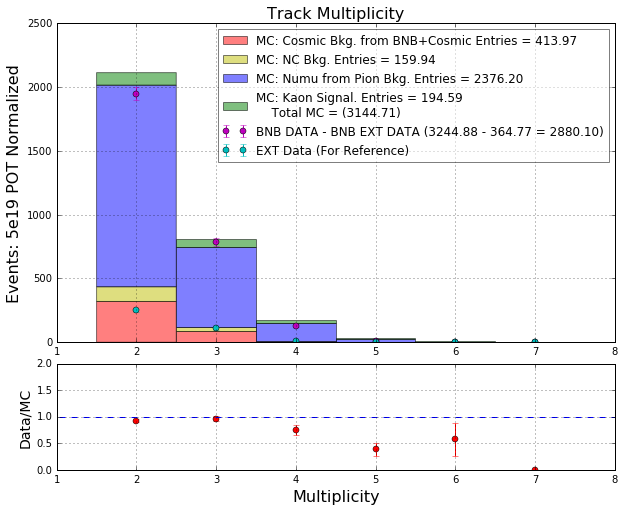
\includegraphics[width=0.9\textwidth]{Figures/kaon_sideband_comp_multiplicity.png} \\
\caption{\textit{The distribution of track multiplicity (number of tracks associated with the interaction) for simulated backgrounds and signal (solid histograms) overlaid with data measurements (``on-beam'' minus ``off-beam'' drawn in purple) for the sideband region in which reconstructed neutrino energy is less than 2.5 GeV. Statistical error bars are drawn on the data points, taking into account statistics from both the ``on-beam'' and ``off-beam'' samples.}}\label{kaon_sideband_comp_multiplicity}
\end{figure}

The next two data to simulation comparisons in the sideband region are shown in Figures \ref{kaon_sideband_comp_phi} and \ref{kaon_sideband_comp_theta}. In these plots, the difference between data and simulation becomes sizable. The first plot is the $\phi$ angle of the muon track associated with the interaction, where $\phi$ is measured in radians with respect to the vertical, around the beam direction. Naively the shape of this distribution should be flat, but the dips at $\pm\frac{\pi}{2}$ correspond to tracks oriented along the drift direction, which are difficult to reconstruct because of the geometry of the sense wires. The second plot is the $\theta$ angle of the muon track, measured with respect to the beam direction. A clear deficit of forward-going tracks (with small $\theta$) can be seen in data, with an excess of vertically-oriented tracks (with $\theta\approx\frac{\pi}{2}$). This difference between data and simulation is particularly important because the high energy $\nu_\mu^{CC}$ interactions which comprise the kaon-enriched signal region have generally very forward-going muons.\\

\begin{figure}[ht!]
\centering
	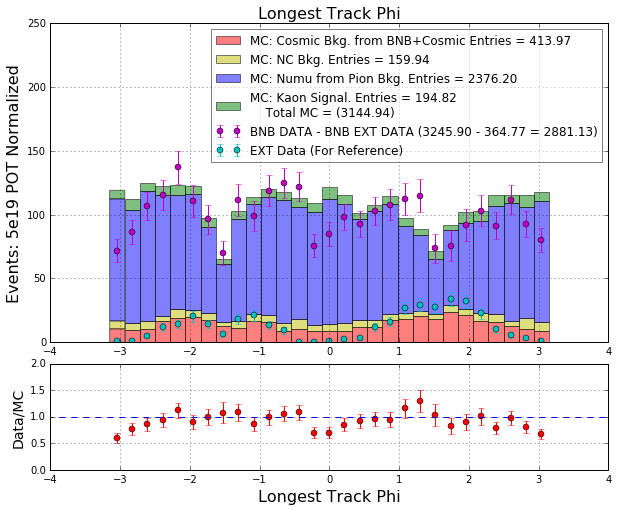
\includegraphics[width=0.9\textwidth]{Figures/kaon_sideband_comp_phi.png} \\
\caption{\textit{The distribution of $\phi$ angle (measured with respect to the vertical) of the longest track associated with the interaction for simulated backgrounds and signal (solid histograms) overlaid with data measurements (``on-beam'' minus ``off-beam'' drawn in purple) for the sideband region in which reconstructed neutrino energy is less than 2.5 GeV. Statistical error bars are drawn on the data points, taking into account statistics from both the ``on-beam'' and ``off-beam'' samples.}}\label{kaon_sideband_comp_phi}
\end{figure}


\begin{figure}[ht!]
\centering
	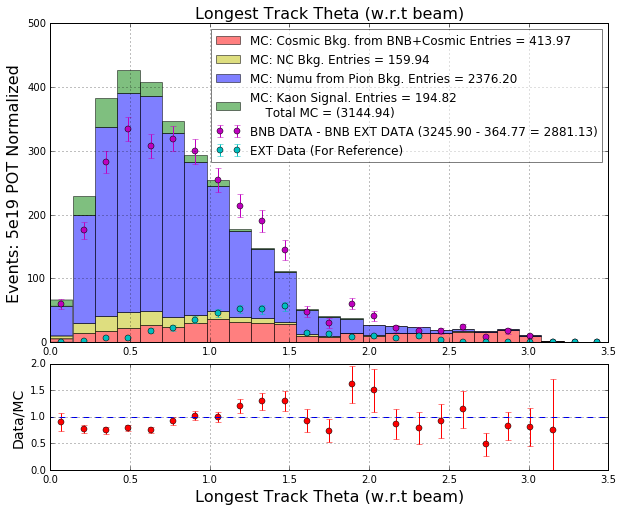
\includegraphics[width=0.9\textwidth]{Figures/kaon_sideband_comp_theta.png} \\
\caption{\textit{The distribution of $\theta$ angle (measured with respect to the beam direction) of the longest track associated with the interaction for simulated backgrounds and signal (solid histograms) overlaid with data measurements (``on-beam'' minus ``off-beam'' drawn in purple) for the sideband region in which reconstructed neutrino energy is less than 2.5 GeV. Statistical error bars are drawn on the data points, taking into account statistics from both the ``on-beam'' and ``off-beam'' samples.}}\label{kaon_sideband_comp_theta}
\end{figure}

The last low level data to simulation comparison is the computed multiple Coulomb scattering (MCS) momentum of the muon track. This distribution includes only tracks with at least one meter contained in the fiducial volume, as having this much track visible is necessary for the MCS technique to work. In this distribution there is a systematic offset in the reconstructed momentum, with that in data being shifted lower than that in simulation. Since MCS momentum is a key ingredient in computing the neutrino energy (Section \ref{kaon_nu_energy_section}), this data to simulation disagreement is particularly important. For this reason, an extensive analysis of the MCS algorithm including data to simulation comparisons was conducted by the author of this thesis. This analysis improved the performance of the algorithm, including an important change to the underlying phenomenological formula not yet discovered by other LArTPC experiments using the MCS technique. This analysis is expected to be published in the Journal of Instrumentation, and the article is included in Chapter \ref{sec:MCS} of this thesis.\\

\begin{figure}[ht!]
\centering
	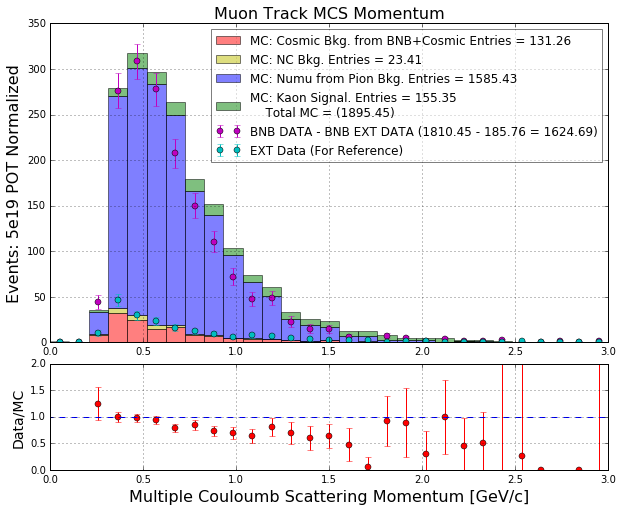
\includegraphics[width=0.9\textwidth]{Figures/kaon_sideband_comp_MCS.png} \\
\caption{\textit{The distribution of multiple Coulomb scattering computed energy for the longest track associated with the interaction for simulated backgrounds and signal (solid histograms) overlaid with data measurements (``on-beam'' minus ``off-beam'' drawn in purple) for the sideband region in which reconstructed neutrino energy is less than 2.5 GeV. Statistical error bars are drawn on the data points, taking into account statistics from both the ``on-beam'' and ``off-beam'' samples.}}\label{kaon_sideband_comp_MCS}
\end{figure}


Despite extensive studies to uncover the underlying causes of the data to simulation disparities and to fix them and/or calibrate them out, the differences remain. Since MicroBooNE is in part an R\&D experiment paving the way for future LArTPC experiments, understanding these differences are a problem that the MicroBooNE collaboration is still working to solve.\\

The comparison of data to simulation in terms of reconstructed neutrino energy for the sideband region is shown in Figure \ref{kaon_stack_sideband_both}. Given the clear systematic shift in energy to lower values in data, any measurement coming from the signal region (which is a small tail at high energies) will have an extremely large systematic uncertainty associated with it. For completeness, the reconstructed energy in the signal region is shown in Figure \ref{kaon_stack_signal_both}. While the referenced SciBooNE result predicts the $K^+$ production rate in simulation is underestimated by a factor of $0.85\pm0.11$ \cite{gary_kaon_production_paper}, the underestimation of data with respect to simulation seen in this analysis is likely not indicative of incorrectly simulated kaon production in the beam-line, but instead due to systematic detector and reconstruction effects that have not yet been solved. %Including an 8\% normalization correction derived from integrating the sideband simulation with respect to data, with 10.8 measured data events in this region, 7.12 expected backgrounds, and 30.75 expected signal events, the kaon production in simulation appears to be underestimated by a factor of
% \begin{equation}
% K^+\text{ rate} = \frac{(10.8 \times 1.08) - 7.12}{30.75} = 0.148
% \end{equation}


\begin{figure}[ht!]
\centering
	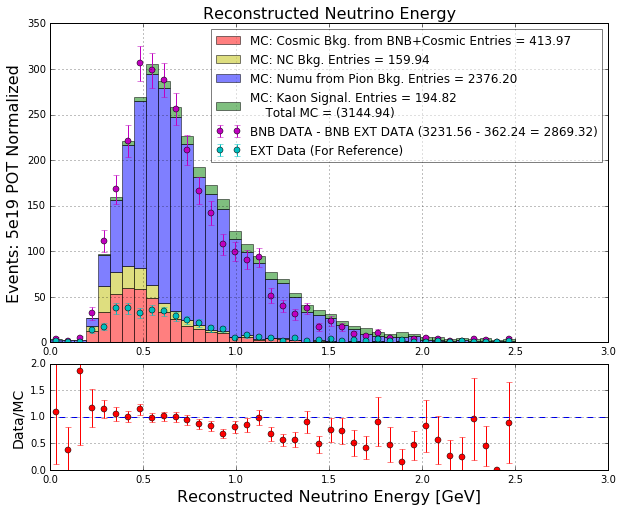
\includegraphics[width=0.9\textwidth]{Figures/kaon_both_sideband.png} \\
\caption{\textit{The distribution of reconstructed neutrino energy for simulated backgrounds and signal (solid histograms) overlaid with data measurements (``on-beam'' minus ``off-beam'' drawn in purple) for the sideband region in which reconstructed neutrino energy is less than 2.5 GeV. Statistical error bars are drawn on the data points, taking into account statistics from both the ``on-beam'' and ``off-beam'' samples.}}\label{kaon_stack_sideband_both}
\end{figure}


\begin{figure}[ht!]
\centering
	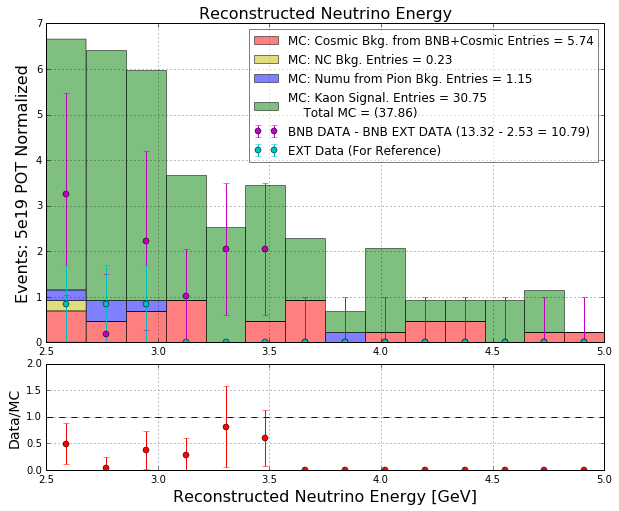
\includegraphics[width=0.9\textwidth]{Figures/kaon_both_signal.png} \\
\caption{\textit{The distribution of reconstructed neutrino energy for simulated backgrounds and signal (solid histograms) overlaid with data measurements (``on-beam'' minus ``off-beam'' drawn in purple) for the signal region in which reconstructed neutrino energy is greater than 2.5 GeV. Statistical error bars are drawn on the data points, taking into account statistics from both the ``on-beam'' and ``off-beam'' samples.}}\label{kaon_stack_signal_both}
\end{figure}

\section{Conclusions}
This thesis chapter has outlined an analysis geared towards measuring the kaon production in the beam-line by MicroBooNE, an important measurement used to constrain a main intrinsic $\nu_e$ background in the electron-like low energy excess search described in Chapter \ref{sec:LEEsensitivity}. Though a similar measurement was previously done by the SciBooNE collaboration, this measurement is important because it is done \textit{in situ} with the same detector that will search for the excess. The method used in this analysis is to select the highest energy $\nu_\mu^{CC}$ interactions within the detector in order to obtain a pure sample of $\nu_\mu$ from $K^+$ decay. The method was demonstrated to be viable in order to make a measurement with comparable significance as that of SciBooNE, though ultimately discrepancies between data and simulation in the analysis were large enough to make an absolute measurement impossible at this time. These differences are still being investigated by the MicroBooNE collaboration, and once they are understood this important analysis can proceed. One of the most important discrepancies lies within the calculation of muon momentum via multiple Coulomb scattering (MCS), since this momentum determination method is the only technique by which the momentum of a muon that exits the TPC can be calculated, and the muons from the high neutrino energy interactions in the kaon enriched signal sample all exit the TPC. A detailed study of the MCS algorithm was conducted by the author of this thesis and has been submitted for publication to the Journal of Instrumentation (JINST). This publication is presented as the following chapter of this thesis.

